\documentclass[10pt,a4paper]{article}
\usepackage[margin=0.7in]{geometry}
\usepackage{multicol}
\usepackage{amsmath}
\usepackage{tikz}
\usepackage{enumitem}
\usepackage{titlesec}
\usepackage{booktabs}
\usepackage{fontspec}

% Compact formatting
\setlength{\columnsep}{0.7cm}
\setlength{\parindent}{0pt}
\setlength{\parskip}{0.12cm}
\titlespacing{\section}{0pt}{0.4cm}{0.15cm}
\titlespacing{\subsection}{0pt}{0.25cm}{0.08cm}
\titlespacing{\subsubsection}{0pt}{0.2cm}{0.05cm}

% Custom section style
\titleformat{\section}{\large\bfseries}{}{0em}{}
\titleformat{\subsection}{\normalsize\bfseries}{}{0em}{}
\titleformat{\subsubsection}{\normalsize\bfseries\itshape}{}{0em}{}

\begin{document}

\begin{center}
{\LARGE \textbf{Consumer Behavior and Utility Theory}}\\[0.15cm]
{\normalsize \textit{Topic 4: Rational Choice, Utility Maximization, and Welfare}}\\[0.15cm]
\hrule
\end{center}
\vspace{-0.3cm}

\begin{multicols}{2}
\footnotesize

% ============================================================================
% PART 1: DEFINITIONS AND CORE CONCEPTS
% ============================================================================
\section*{1. Definition and Foundational Concepts}

\subsection*{Consumer Behavior}
\textbf{Consumer Behavior} is the study of how individuals make decisions to allocate their limited resources (income, time) among competing goods and services to maximize \textbf{satisfaction} or \textbf{utility}. It forms the microeconomic foundation of the demand curve.

\textbf{Key Questions Addressed:}
\begin{itemize}[leftmargin=*,nosep]
    \item Why does a consumer buy more of a good when its price falls?
    \item How does a consumer choose between two goods given a budget constraint?
    \item What is the welfare gain a consumer receives from market transactions?
\end{itemize}

\subsection*{Utility -- Basic Concept}
\textbf{Utility} ($U$) is the satisfaction, happiness, or pleasure a consumer derives from consuming a good or service. It is a \textbf{subjective} and psychological concept, not an objective physical measure. Economists assume consumers act \textit{as if} they maximize utility.

\textbf{Two Approaches to Measuring Utility:}
\begin{enumerate}[leftmargin=*,nosep]
    \item \textbf{Cardinal Utility:} Utility is \textbf{measurable} in numerical units (``utils''). One can say: ``Bundle A gives 80 utils, Bundle B gives 50 utils, so I prefer A exactly 1.6 times as much.'' This is the classical approach (Marshall, Pigou). Assumes interpersonal comparisons are possible.
    \item \textbf{Ordinal Utility:} Utility is \textbf{not measurable} cardinally; consumers can only \textbf{rank} bundles in order of preference (1st, 2nd, 3rd...). One can say: ``I prefer A to B,'' but not by how much. This is the modern approach (Hicks-Allen, Samuelson). Uses indifference curves and budget lines.
\end{enumerate}

\subsection*{Consumer's Preference Ordering (Ordinal Approach)}
Consumers are assumed to have a rational preference relation $\succsim$ (``at least as good as'') satisfying:
\begin{enumerate}[leftmargin=*,nosep]
    \item \textbf{Completeness:} For any two bundles $A$ and $B$, the consumer can say $A \succsim B$ or $B \succsim A$ (or both, meaning indifference). No indecision.
    \item \textbf{Transitivity:} If $A \succsim B$ and $B \succsim C$, then $A \succsim C$. Preferences are logically consistent.
    \item \textbf{Monotonicity (Non-satiation):} More of a good is always preferred to less (``more is better''), assuming goods are ``goods'' not ``bads.''
    \item \textbf{Convexity:} Averages are preferred to extremes. The consumer prefers a mix of goods rather than extreme bundles (diminishing MRS).
\end{enumerate}

% ============================================================================
% PART 2: MEMORY TRIGGERS
% ============================================================================
\section*{2. How to Remember (Conceptual Anchors)}

\begin{itemize}[leftmargin=*,nosep]
    \item \textbf{Cardinal = Countable (like Calories):} ``Cardinal'' shares root with ``cardinal numbers'' (1, 2, 3...). Think of utils as countable satisfaction points.
    \item \textbf{Ordinal = Order (like Olympic Medals):} You only know Gold > Silver > Bronze, not how much better. Ranking, not measuring.
    \item \textbf{Total Utility (TU) = Total Happiness from all units consumed.} Marginal Utility (MU) = \textbf{Extra} happiness from one \textbf{more} unit. (M for Marginal = More.)
    \item \textbf{Diminishing MU:} The first slice of pizza is heavenly; the 5th slice makes you sick. Each additional unit adds less satisfaction than the previous one.
    \item \textbf{Equimarginal Principle:} Allocate your budget so the ``bang for your buck'' ($MU/P$) is \textbf{equal} across all goods. Mnemonic: ``Balance your bucks for maximum bliss.''
    \item \textbf{Income Effect vs Substitution Effect:}
    \begin{itemize}[nosep]
        \item Price falls $\to$ you feel \textbf{richer} (real income $\uparrow$) $\to$ buy more normal goods = \textbf{Income Effect}.
        \item Price falls $\to$ good is \textbf{cheaper relative} to others $\to$ switch toward it = \textbf{Substitution Effect}.
    \end{itemize}
    \item \textbf{Slutsky Equation:} Total Effect = Substitution Effect (always negative for own-price) + Income Effect (sign depends on normal/inferior good). ``Slutsky Separates the Slopes.''
    \item \textbf{Consumer Surplus = Bargain Joy:} The difference between what you \textit{would} have paid and what you \textit{actually} paid. The area below demand curve, above price. ``The joy of a good deal.''
\end{itemize}

% ============================================================================
% PART 3: MATHEMATICAL FRAMEWORK
% ============================================================================
\section*{3. Mathematical Formulation and Concepts}

\subsection*{Cardinal Utility: Total and Marginal Utility}

Let $U(x)$ be the total utility from consuming $x$ units of a good. \textbf{Marginal Utility} is the additional utility from consuming one more unit:

\[
MU_x = \frac{\Delta TU}{\Delta x} \quad \text{(Discrete)} \qquad MU_x = \frac{dU}{dx} \quad \text{(Continuous)}
\]

\textbf{Relationship between TU and MU:}
\begin{itemize}[leftmargin=*,nosep]
    \item When $MU > 0$, TU is \textbf{increasing}.
    \item When $MU = 0$, TU is at its \textbf{maximum} (satiation point).
    \item When $MU < 0$, TU is \textbf{decreasing} (disutility).
    \item The slope of the TU curve at any point equals the value of MU at that quantity.
\end{itemize}

\textbf{Law of Diminishing Marginal Utility (Gossen's First Law):}
As a consumer consumes successive units of a good, the marginal utility derived from each additional unit eventually \textbf{declines}, \textit{ceteris paribus}.
\[
\frac{d(MU)}{dx} = \frac{d^2 U}{dx^2} < 0
\]
\textit{Example:} The first glass of water when thirsty gives immense satisfaction (high MU); the second gives less; the fifth may give zero or negative MU.

\subsection*{Equimarginal Principle (Gossen's Second Law, Consumer Equilibrium)}

A consumer with income $M$ facing prices $P_x, P_y$ maximizes utility when:
\[
\frac{MU_x}{P_x} = \frac{MU_y}{P_y} = \lambda \quad \text{(Marginal Utility of Money)}
\]
Subject to: $P_x \cdot x + P_y \cdot y = M \quad \text{(Budget Constraint)}$.

\textbf{Intuition:} The last dollar spent on each good must yield the same additional satisfaction. If $MU_x/P_x > MU_y/P_y$, the consumer should reallocate spending from $y$ to $x$ to increase total utility.

\textbf{For $n$ goods:}
\[
\frac{MU_1}{P_1} = \frac{MU_2}{P_2} = \dots = \frac{MU_n}{P_n} = \lambda
\]

\subsection*{Ordinal Utility: Indifference Curves and MRS}

An \textbf{indifference curve} represents all combinations of two goods that give the consumer the same level of utility. \textbf{Marginal Rate of Substitution (MRS)} is the slope of the indifference curve:

\[
MRS_{xy} = -\frac{dy}{dx}\bigg|_{U=\text{const}} = \frac{MU_x}{MU_y}
\]

The consumer maximizes utility where the budget line is \textbf{tangent} to the highest attainable indifference curve:
\[
MRS_{xy} = \frac{P_x}{P_y} \quad \text{and} \quad P_x x + P_y y = M
\]

\subsection*{Substitution Effect, Income Effect, and the Slutsky Equation}

When the price of good $x$ falls ($P_x \downarrow$), two effects occur:

\textbf{(1) Substitution Effect ($\Delta x^s$):} The good is now relatively cheaper. Consumer substitutes \textit{toward} $x$ and away from $y$. This effect is \textbf{always negative} for own-price changes (i.e., consumption of $x$ rises when its price falls).

\textbf{(2) Income Effect ($\Delta x^i$):} The consumer's \textbf{real income} (purchasing power) increases because the same money income can buy more goods. Effect on $x$ depends on good type:
\begin{itemize}[nosep]
    \item \textbf{Normal good:} Income effect is positive ($\uparrow$ real income $\to$ $\uparrow$ consumption $x$). Reinforces substitution effect.
    \item \textbf{Inferior good:} Income effect is negative. Offsets substitution effect.
    \item \textbf{Giffen good:} Negative income effect is so strong it outweighs the substitution effect, leading to upward-sloping demand! (Very rare.)
\end{itemize}

\textbf{The Slutsky Equation (Elasticity Form):}
\[
\underbrace{\frac{\partial x}{\partial P_x}}_{\text{Total Effect}} = \underbrace{\frac{\partial x^c}{\partial P_x}}_{\text{Subst. Effect } (-)} - \underbrace{x \cdot \frac{\partial x}{\partial M}}_{\text{Income Effect}}
\]
Where $x^c$ is compensated (Hicksian) demand. Multiplying both sides by $P_x/x$ gives the elasticity form:
\[
\varepsilon_{xx} = \varepsilon_{xx}^c - s_x \cdot \eta_x
\]
Where:
\begin{itemize}[leftmargin=*,nosep]
    \item $\varepsilon_{xx}$ = Uncompensated (Marshallian) own-price elasticity.
    \item $\varepsilon_{xx}^c$ = Compensated (Hicksian) own-price elasticity (\textbf{always negative}).
    \item $s_x = P_x x / M$ = Budget share of good $x$.
    \item $\eta_x$ = Income elasticity of demand for good $x$.
\end{itemize}

\textbf{From Slutsky equation, compute elasticities:}
If we know compensated elasticity, budget share, and income elasticity, we can derive Marshallian elasticity. For example: Given $\varepsilon_{xx}^c = -1.2$, $s_x = 0.3$, $\eta_x = 0.8$:
\[
\varepsilon_{xx} = -1.2 - (0.3 \times 0.8) = -1.2 - 0.24 = -1.44
\]
(Marshallian demand more elastic than Hicksian because good is normal; income effect reinforces.)

\subsection*{Consumer's Surplus (Marshallian)}

\textbf{Consumer Surplus (CS)} is the difference between the \textbf{maximum amount a consumer is willing to pay} (total utility) and what they \textbf{actually pay} (market price $\times$ quantity).

\[
CS = \int_{0}^{Q^*} P(Q) \, dQ - P^* \cdot Q^*
\]
For a linear demand $P = a - bQ$, with market price $P^*$:
\[
CS = \frac{1}{2} \times (\text{Choke Price} - P^*) \times Q^* = \frac{1}{2} \cdot \frac{(a - P^*)^2}{b}
\]

\textbf{Applications:}
\begin{itemize}[leftmargin=*,nosep]
    \item Measuring welfare gains from trade, price reductions, or new goods.
    \item Evaluating public projects: Cost-Benefit Analysis.
    \item Determining optimal taxation and deadweight loss.
    \item Setting price discrimination strategies (capturing consumer surplus).
\end{itemize}

% ============================================================================
% PART 4: GRAPHICAL ANALYSIS
% ============================================================================
\section*{4. Graphical Illustrations}

\subsection*{Total Utility and Marginal Utility Curves}
\begin{center}
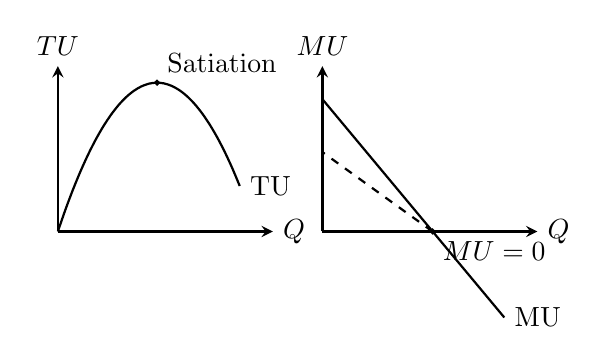
\begin{tikzpicture}[scale=0.42, thick, >=stealth]
    % TU
    \draw[->] (0,0) -- (6.5,0) node[right] {$Q$};
    \draw[->] (0,0) -- (0,5) node[above] {$TU$};
    \draw[thick, domain=0:5.5, smooth] plot (\x, {4 - 1.5*(\x-3)*(\x-3)/3 + 0.5}) node[right] {TU};
    \filldraw (3,4.5) circle (1.5pt) node[above right] {Satiation};
    % MU
    \draw[->] (8,0) -- (14.5,0) node[right] {$Q$};
    \draw[->] (8,0) -- (8,5) node[above] {$MU$};
    \draw[thick, domain=8:13.5, smooth] plot (\x, {4 - 1.2*(\x-8)}) node[right] {MU};
    \filldraw (11.33,0) circle (1.5pt) node[below right] {$MU=0$};
    \draw[dashed] (11.33,0) -- (8,2.4);
\end{tikzpicture}
\end{center}
\textit{Interpretation:} As $Q$ increases, $TU$ rises at a decreasing rate (while $MU>0$), reaches maximum ($MU=0$), then falls ($MU<0$). The $MU$ curve is the derivative (slope) of the $TU$ curve.

\subsection*{Consumer Equilibrium: Cardinal Approach}
\begin{center}
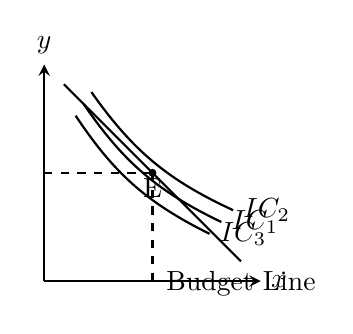
\begin{tikzpicture}[scale=0.5, thick, >=stealth]
    \draw[->] (0,0) -- (5.5,0) node[right] {$x$};
    \draw[->] (0,0) -- (0,5.5) node[above] {$y$};
    \draw[thick] (0.5,5) -- (5,0.5) node[below] {Budget Line};
    \draw[thick] (1,4.5) to[bend right=15] (4.5,1.5) node[right] {$IC_1$};
    \draw[thick] (1.2,4.8) to[bend right=15] (4.8,1.8) node[right] {$IC_2$};
    \draw[thick] (0.8,4.2) to[bend right=15] (4.2,1.2) node[right] {$IC_3$};
    \filldraw (2.75,2.75) circle (2pt);
    \node at (2.75,2.35) {E};
    \draw[dashed] (2.75,0) -- (2.75,2.75);
    \draw[dashed] (0,2.75) -- (2.75,2.75);
\end{tikzpicture}
\end{center}
\textit{At $E$:} $MRS = P_x/P_y$; budget exhausted; consumer on highest attainable indifference curve ($IC_2$).

\subsection*{Substitution and Income Effects (Normal Good)}
\begin{center}
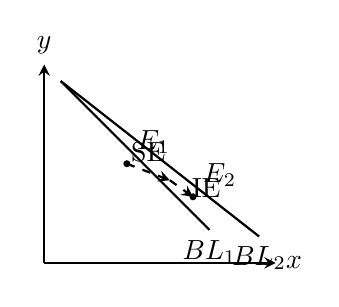
\begin{tikzpicture}[scale=0.42, thick, >=stealth]
    \draw[->] (0,0) -- (7,0) node[right] {$x$};
    \draw[->] (0,0) -- (0,6) node[above] {$y$};
    % Original BL
    \draw (0.5,5.5) -- (5,1) node[below] {$BL_1$};
    % New BL (Px fell)
    \draw (0.5,5.5) -- (6.5,0.8) node[below] {$BL_2$};
    % Tangency points
    \filldraw (2.5,3) circle (2pt) node[above right] {$E_1$};
    \filldraw (4.5,2) circle (2pt) node[above right] {$E_2$};
    % Arrows
    \draw[->, dashed] (2.5,3) -- (3.8,2.5) node[midway, above] {SE};
    \draw[->, dashed] (3.8,2.5) -- (4.5,2) node[midway, right] {IE};
\end{tikzpicture}
\end{center}
\textit{Normal Good:} Total effect ($E_1 \to E_2$) = Substitution Effect (always increases $x$) + Income Effect (also increases $x$).

% ============================================================================
% PART 5: DEEPENED CONCEPTS
% ============================================================================
\section*{5. Deepened Theoretical Concepts}

\subsection*{Slutsky vs. Hicksian Compensation}
\begin{itemize}[leftmargin=*,nosep]
    \item \textbf{Slutsky compensation:} After price change, the consumer is given enough income to buy the \textit{original bundle} at new prices. The substitution effect is measured along a rotated budget line through the original bundle.
    \item \textbf{Hicksian compensation:} After price change, income is adjusted so the consumer remains on the \textit{same indifference curve}. Yields the \textit{pure} substitution effect.
\end{itemize}
For small price changes, both measures converge. Slutsky is observable and used empirically.

\subsection*{Law of Demand: Revisited via Slutsky}
The Law of Demand states: $\partial x / \partial P_x < 0$ (demand curve slopes down). The Slutsky equation shows this holds \textbf{as long as the income effect is not negative and large enough to outweigh the substitution effect}. For a normal good, both effects reinforce -- Law of Demand \textbf{must} hold. For an inferior good, the income effect opposes; if it dominates, we get a \textbf{Giffen good} -- theoretically possible but empirically exceptionally rare.

\subsection*{Consumer's Surplus: Detailed Computation}
For a non-linear demand $Q = f(P)$, consumer surplus is the definite integral:
\[
CS = \int_{P^*}^{P_{\text{max}}} Q(P) \, dP
\]
\textit{Example:} Demand $Q = 100/P^2$. Market price $P^* = 5$, choke price $\infty$ technically, but integrate from 5 to some high value or compute area.

% ============================================================================
% PART 6: EXTENSIVE CASE STUDIES
% ============================================================================
\section*{6. Comprehensive Case Studies}

\subsection*{Case Study 1: The Giffen Good Phenomenon – Potatoes in the Irish Famine (1845--1852)}

\textbf{Background:} During the Great Irish Famine, the staple food of the poor was the potato. When potato prices rose dramatically due to the blight destroying crops, Sir Robert Giffen (and later Alfred Marshall) observed a paradoxical behavior: poor households \textit{increased} their consumption of potatoes as prices rose, contradicting the Law of Demand. This became the classic textbook example of a \textbf{Giffen good}.

\textbf{Economic Mechanism (Detailed Slutsky Decomposition):}

Consider a poor household consuming two goods: \textbf{Potatoes (P)} -- a staple, inferior good that consumes a large share of the budget -- and \textbf{Meat (M)} -- a luxury, normal good.

\textit{Initial Situation:} Household income = \$10/week. Potatoes cost \$1/kg, Meat costs \$5/kg. Baseline consumption: 7 kg potatoes (\$7), 0.6 kg meat (\$3).

\textit{Shock:} Potato blight destroys crops. Potato price rises to \$3/kg.

\textbf{Step 1: Substitution Effect.}
Potatoes are now relatively more expensive compared to meat. Holding real income constant (compensated), the household would substitute \textit{away} from potatoes toward meat. The substitution effect on potato consumption is \textbf{negative}: the household wants fewer potatoes. $\Delta x^s < 0$.

\textbf{Step 2: Income Effect.}
The price increase causes a massive reduction in \textbf{real income}. The household's purchasing power collapses. Before, \$10 bought 7 kg potato + 0.6 kg meat. Now, 7 kg potatoes alone would cost \$21 -- \textbf{more than their entire income}. The household is now substantially poorer.

Because potatoes are an \textbf{inferior good} and consume a very large share of the budget, the income effect is \textbf{positive and very large} (poverty forces the household to buy more inferior staple foods). $\Delta x^i > 0$ and $|\Delta x^i| > |\Delta x^s|$.

\textbf{Step 3: Total Effect.}
\[
\Delta x = \Delta x^s + \Delta x^i
\]
Since $|\Delta x^i| > |\Delta x^s|$, the total effect is \textbf{positive}: $\Delta x > 0$. The household ends up consuming \textit{more} potatoes despite the price rise. Meat becomes completely unaffordable, so the household cuts meat entirely and spends even more of its remaining budget on the now-expensive but still cheapest calorie source: potatoes.

\textbf{Slutsky Equation Application:}
\[
\varepsilon_{PP} = \varepsilon_{PP}^c - s_P \cdot \eta_P
\]
Assume: $\varepsilon_{PP}^c = -0.8$ (compensated elasticity), $s_P = 0.7$ (potatoes are 70\% of budget), $\eta_P = -1.5$ (highly inferior -- income elasticity is negative).
\[
\varepsilon_{PP} = -0.8 - (0.7 \times (-1.5)) = -0.8 + 1.05 = +0.25
\]
Marshallian own-price elasticity is \textbf{positive} ($+0.25$), violating the Law of Demand! A 1\% price increase leads to a 0.25\% \textit{increase} in quantity demanded -- a Giffen good.

\textbf{Conditions for a Giffen Good (All must hold):}
\begin{enumerate}[leftmargin=*,nosep]
    \item The good must be \textbf{strongly inferior} ($\eta < 0$ with large magnitude).
    \item The good must consume a \textbf{large share of the budget} ($s$ must be large).
    \item There must be \textbf{no close substitutes} (otherwise substitution effect would be large).
    \item Applies to poor consumers facing a \textbf{subsistence constraint}.
\end{enumerate}

\textbf{Modern Empirical Evidence:} Jensen and Miller (2008, \textit{American Economic Review}) found evidence of Giffen behavior among extremely poor households in rural China. When the price of rice (staple) was subsidized, households \textit{reduced} rice consumption (as real income rose, they bought more meat). When subsidies were removed and rice price rose, very poor households consumed \textit{more} rice and cut meat consumption. This is the first rigorous empirical confirmation of Giffen behavior.

\textbf{Economic Lesson:} The law of demand is not absolute; it depends on the relative magnitudes of substitution and income effects. Giffen behavior highlights the critical role of income constraints and inferior goods in consumer theory. It also demonstrates why economics distinguishes between theoretical possibilities and empirical regularities.

\subsection*{Case Study 2: Consumer Surplus and the Value of Digital Goods – The Case of Google Search}

\textbf{Background:} Many digital goods (search engines, social media, maps) are provided to consumers at a \textbf{zero monetary price}. GDP and traditional economic metrics fail to capture the value consumers derive from these services because no market transaction occurs. Consumer surplus estimation becomes crucial for measuring welfare in the digital economy.

\textbf{The Problem: How much is ``free'' Google Search worth to consumers?}

\textbf{Methodology: Estimating Consumer Surplus for a Zero-Price Good}

Economists Brynjolfsson, Eggers, and Gannamaneni (2019) used massive online choice experiments to measure the value of digital goods.

\textit{Approach:} They asked representative samples of consumers: ``What is the minimum amount of money you would accept to give up using Google Search for one month?'' This represents the \textbf{compensating variation} -- the income adjustment needed to keep utility unchanged when the good is removed.

\textit{Alternatively:} Infer the demand curve indirectly. Even though the monetary price is zero, the ``full price'' includes \textbf{time costs, attention costs, and privacy costs}. By observing how usage changes with variations in these non-monetary costs (or hypothetical monetary prices in surveys), one can trace out a demand curve.

\textbf{Demand Estimation and Surplus Calculation:}

Assume a survey reveals the following (hypothetical, stylized) demand schedule for Google Search:

\begin{center}
\begin{tabular}{@{ }c@{ }c@{ }}
\toprule
\textbf{Monthly Price (\$)} & \textbf{Users (Millions)} \\
\midrule
\$50  & 10 \\
\$30  & 40 \\
\$20  & 80 \\
\$10  & 150 \\
\$5   & 220 \\
\$0   & 280 \\
\bottomrule
\end{tabular}
\end{center}

\textit{Linear Approximation:} $Q = 280 - 5P$. The choke price (where $Q=0$) is $P_{\text{max}} = 56$.

\[
CS = \int_{0}^{280} \left(56 - \frac{Q}{5}\right) dQ - 0 \times 280 = \frac{1}{2} \times 56 \times 280
\]
\[
CS \approx \mathbf{\$7,840 \text{ million}} = \mathbf{\$7.84 \text{ billion per month}}
\]
Annual consumer surplus from Google Search alone would be on the order of \textbf{\$90+ billion}. This value is \textbf{not captured in GDP} because no transaction occurs. The actual estimates by Brynjolfsson et al. for all free digital goods (search, email, maps, social media) reach several \textbf{hundreds of billions of dollars annually} -- essentially equivalent to a substantial fraction of GDP.

\textbf{Applications and Policy Implications:}
\begin{enumerate}[leftmargin=*,nosep]
    \item \textbf{GDP Mismeasurement:} Massive consumer welfare is generated without any monetary exchange, leading to underestimation of economic well-being and productivity growth in the digital age.
    \item \textbf{Antitrust/Regulation:} If a dominant platform (like Google) were to degrade quality or charge fees, the consumer surplus loss would be enormous. Regulators must weigh this against potential harms when considering break-ups or restrictions.
    \item \textbf{Digital Divide:} Lower-income individuals receive disproportionately large consumer surplus from free digital goods (since they pay zero), reducing effective inequality (real consumption inequality is lower than money-income inequality).
    \item \textbf{Privacy Trade-off:} These services are funded by advertising revenue, which relies on user data. The ``price'' consumers pay is in the form of personal data and attention (non-monetary costs). Consumer surplus analysis must incorporate the \textbf{disutility of privacy loss} as a reduction in net surplus.
    \item \textbf{Cost-Benefit of Internet Access Programs:} Government subsidies for broadband access can be justified by the large consumer surplus generated by access to digital services.
\end{enumerate}

\textbf{Economic Concept Summary:} Consumer surplus is a powerful tool to measure welfare for goods that exist outside traditional markets. In the modern economy, understanding and measuring consumer surplus is increasingly important for policy evaluation, regulation of tech platforms, and assessing real economic well-being beyond GDP metrics.

\columnbreak

% ============================================================================
% PART 7: EXAM QUESTIONS
% ============================================================================
\section*{7. Exam Practice Questions \& Model Answers}

\subsection*{Question 1: Utility Maximization (Cardinal)}
\textbf{A consumer has utility function $U = 10x^{0.5} + 5y$. Prices: $P_x = 2$, $P_y = 4$. Income = \$60.}
\textbf{(a) Find the consumer's optimal consumption bundle.}
\textbf{(b) Verify the equimarginal principle at the optimum.}
\textbf{(c) If $P_x$ falls to \$1, decompose the total change into substitution and income effects.}

\vspace{0.1cm}
\textbf{Solution:}
\textbf{(a)} $MU_x = \frac{10}{2\sqrt{x}} = \frac{5}{\sqrt{x}}$, $MU_y = 5$.
Equimarginal: $\frac{MU_x}{P_x} = \frac{MU_y}{P_y} \Rightarrow \frac{5/\sqrt{x}}{2} = \frac{5}{4} \Rightarrow \frac{5}{2\sqrt{x}} = \frac{5}{4} \Rightarrow 2\sqrt{x} = 4 \Rightarrow \sqrt{x}=2 \Rightarrow \mathbf{x=4}$.
Budget: $2(4) + 4y = 60 \Rightarrow 8 + 4y = 60 \Rightarrow 4y=52 \Rightarrow \mathbf{y=13}$.
Optimal bundle: $\mathbf{(4, 13)}$.

\textbf{(b)} At optimum: $\frac{MU_x}{P_x} = \frac{5/\sqrt{4}}{2} = \frac{2.5}{2} = 1.25$. $\frac{MU_y}{P_y} = \frac{5}{4} = 1.25$. Equal. $\checkmark$

\vspace{0.05cm}
\textbf{(c) New $P_x=1$, New Budget: $x + 4y = 60$.}
New optimum: $\frac{5/\sqrt{x}}{1} = \frac{5}{4} \Rightarrow \frac{5}{\sqrt{x}} = 1.25 \Rightarrow \sqrt{x} = 4 \Rightarrow \mathbf{x=16}$. Budget: $16 + 4y = 60 \Rightarrow 4y=44 \Rightarrow \mathbf{y=11}$. New bundle: $\mathbf{(16, 11)}$.
\textit{Total Effect on x:} $\Delta x = 16 - 4 = +12$.

To decompose: At new prices, find income needed to buy original bundle (Slutsky): $M' = 1(4) + 4(13) = 4 + 52 = 56$. At $M'=56$, find demand: $\frac{5/\sqrt{x}}{1} = \frac{5}{4} \Rightarrow x=16$ (same condition, as demand for $x$ with this utility is independent of income! MU of $y$ is constant, so $x$ depends only on prices). Thus, \textbf{Substitution Effect} = $16 - 4 = 12$. \textbf{Income Effect} = $0$ (because $MU_y$ constant $\to$ quasi-linear utility; all of change is due to price change, none from income). This is a \textbf{zero income effect} good.

\vspace{0.2cm}

\subsection*{Question 2: Slutsky Equation Application}
\textbf{The demand for gasoline is $Q = 100 - 2P$. Original price $P_0 = 10$. New price $P_1 = 15$. Income = \$500.}
\textbf{(a) Calculate the uncompensated (Marshallian) price elasticity at $P_0$.}
\textbf{(b) If the compensated (Hicksian) elasticity is estimated at $-0.2$, and gasoline's budget share is 0.04, what is the implied income elasticity using the Slutsky equation? Is gasoline a normal or inferior good?}

\vspace{0.1cm}
\textbf{Solution:}
\textbf{(a)} At $P_0=10$: $Q = 100 - 2(10) = 80$. $dQ/dP = -2$. $\varepsilon_{xx} = -2 \times (10/80) = \mathbf{-0.25}$.

\textbf{(b)} Slutsky: $\varepsilon_{xx} = \varepsilon_{xx}^c - s_x \cdot \eta_x$.
$-0.25 = -0.2 - 0.04 \cdot \eta_x \Rightarrow -0.05 = -0.04 \cdot \eta_x \Rightarrow \eta_x = \mathbf{1.25}$.
Since $\eta_x > 0$, gasoline is a \textbf{normal good} (more specifically, a luxury since $\eta_x > 1$). The income effect reinforces the substitution effect, making Marshallian demand more elastic ($-0.25$) than Hicksian demand ($-0.2$).

\vspace{0.2cm}

\subsection*{Question 3: Consumer Surplus}
\textbf{Demand for event tickets: $P = 200 - 0.5Q$. Supply is perfectly elastic at $P=50$.}
\textbf{(a) Find equilibrium quantity and consumer surplus.}
\textbf{(b) If the government imposes a tax of \$30 per ticket (suppliers collect), calculate the new consumer surplus, tax revenue, and deadweight loss.}

\vspace{0.1cm}
\textbf{Solution:}
\textbf{(a)} At $P=50$: $50 = 200 - 0.5Q \Rightarrow 0.5Q = 150 \Rightarrow Q^* = 300$.
Choke price: $Q=0 \Rightarrow P=200$. $CS = 0.5 \times (200-50) \times 300 = 0.5 \times 150 \times 300 = \mathbf{\$22,500}$.

\textbf{(b)} \$30 tax shifts supply up to $P=80$ (suppliers must receive 80 to keep 50 after tax). New equilibrium: $80 = 200 - 0.5Q \Rightarrow Q=240$. New $CS = 0.5 \times (200-80) \times 240 = 0.5 \times 120 \times 240 = \mathbf{\$14,400}$.
Tax revenue = $30 \times 240 = \mathbf{\$7,200}$.
Deadweight loss = $0.5 \times 30 \times (300-240) = 0.5 \times 30 \times 60 = \mathbf{\$900}$.
Check: Original $CS$ (22,500) = New $CS$ (14,400) + Tax Revenue (7,200) + DWL (900) = 22,500. $\checkmark$

\vspace{0.2cm}

\subsection*{Question 4: Conceptual}
\textbf{Explain why the substitution effect of a price change is always negative (i.e., quantity demanded moves opposite to the direction of price change), even for Giffen goods.}

\vspace{0.1cm}
\textbf{Answer:} The substitution effect isolates the change in consumption due purely to the change in \textbf{relative prices}, holding real income (utility) constant. When a good becomes relatively cheaper, rationality requires that a consumer substitutes \textit{toward} the now-cheaper good and \textit{away} from relatively more expensive goods to maintain the same utility level. This stems from convexity of indifference curves (diminishing MRS) -- the slope of the curve flattens as we move along it, and tangency with a flatter budget line (due to lower relative price) must occur at a higher quantity of the cheaper good. For a Giffen good, the substitution effect is still negative; however, the income effect is positive (the good is inferior) and so large in magnitude that it dominates the negative substitution effect, creating a positive total effect. The substitution effect itself never violates the law of demand.

\end{multicols}

% ============================================================================
% SUMMARY TABLE
% ============================================================================
\vspace{0.3cm}
\begin{center}
\fbox{\begin{minipage}{0.9\textwidth}
\footnotesize
\textbf{Summary Cheat Sheet: Consumer Theory \& Utility}
\begin{center}
\begin{tabular}{@{}p{3.2cm}p{2.8cm}p{3.2cm}@{}}
\toprule
\textbf{Concept} & \textbf{Formula/Condition} & \textbf{Key Insight} \\
\midrule
Marginal Utility & $MU = \Delta TU / \Delta Q$ & Slope of TU curve \\
Diminishing MU & $d(MU)/dQ < 0$ & Each additional unit adds less satisfaction \\
Equimarginal Principle & $MU_x/P_x = MU_y/P_y$ & Last dollar yields same marginal utility across all goods \\
MRS & $MRS = MU_x/MU_y$ & Slope of indifference curve; willingness to trade \\
Utility Max (Ordinal) & $MRS = P_x/P_y$ & Tangency of BL and IC \\
Slutsky Equation & $\varepsilon = \varepsilon^c - s \cdot \eta$ & Total = Substitution (always $-$) + Income Effect \\
Consumer Surplus & $CS = \int_P^{P_{max}} Q(P)\,dP$ & Welfare measure; area under demand, above price \\
Giffen Good & $\varepsilon > 0$ (positive) & Strong inferior good with large budget share; IE dominates SE \\
\bottomrule
\end{tabular}
\end{center}

\vspace{0.1cm}
\textbf{Quick Sign Summary:}
\begin{itemize}[leftmargin=*,nosep]
    \item Substitution Effect: \textbf{always negative} ($\partial x^c / \partial P_x < 0$).
    \item Income Effect for Normal Good: negative ($-\partial x/\partial M < 0$, so IE negative, reinforces SE).
    \item Income Effect for Inferior Good: positive (offsets SE).
    \item Consumer Surplus increases when price falls; decreases when price rises.
\end{itemize}
\end{minipage}}
\end{center}

\end{document}